\documentclass{resume} % Use the custom resume.cls style
\usepackage{graphicx}
\graphicspath{ {./images/} }

\usepackage[left=0.4 in,top=0.4in,right=0.4 in,bottom=0.4in]{geometry} % Document margins
\newcommand{\tab}[1]{\hspace{.2667\textwidth}\rlap{#1}} 
\newcommand{\itab}[1]{\hspace{0em}\rlap{#1}}
\name{Robert Rothschild}
\address{rarothsc@gmail.com, (720)-785-0488 \\
2137 Superior St. Bellingham WA, 98229}

\begin{document}

%-------------------------------------------------
%	OBJECTIVE
%-------------------------------------------------

\begin{rSection}{OBJECTIVE}

{To find a job that allows me to exercise my strength and knowledge in software engineering.}

\end{rSection}
%-------------------------------------------------
%	EDUCATION SECTION
%-------------------------------------------------

\begin{rSection}{Education}

{\bf Bachelor of Science in Engineering} \hfill {2014 - 2018}
\\ 
Fort Lewis College, Durango CO

\end{rSection}

%-------------------------------------------------
%	EXPERIENCE SECTION
%-------------------------------------------------

\begin{rSection}{EXPERIENCE}

{\textbf{Engineer - The Heliospace Corporation} \hfill Jan 2017 - Current \\
Lead the company's software development effort including the creating of an API for processing Finite Element Analysis data. Maintained databases used for writing out various engineering documents such as bill of materials and material identification and usage list. Wrote and contributed to numerous technical documents given to customers. Has been on multiple hardware integration and test teams for projects such as the James Webb Space Telescope and NASA's Lunar Gateway.}

{\textbf{Research Assistant - Colorado Space Grant Consortium} \hfill Jan 2016 - May 2018 \\
Participated in the robotics challenge to design, fabricate, and program a robot capable of traversing a Mars like environment. }

{\textbf{Research Assistant - Fort Lewis College} \hfill May 2015 - July 2015 \\
Responsible for collecting marine data using autonomous boats and processing the data in MatLab.}

\end{rSection} 


%-------------------------------------------------
%	SKILLS SECTION
%-------------------------------------------------
\begin{rSection}{SKILLS}

\begin{tabular}{ @{} >{\bfseries}l @{\hspace{6ex}} l }
Skills & Quick learner, self starter, people and time management, innovative and creative thinking,\\ & risk management, ambitious, responsible, and well disciplined
\\
\end{tabular}

\begin{table}[h]
    \centering
    \begin{tabular}{ c c c c c c c c }
    \centering
    \setlength\extrarowheight{2.5pt} 
    Django & Python & HTML & Css & GCP & MatLab & LaTeX & MS Office \\ 
    
\includegraphics[width=0.05\textwidth]{logoDjango} & 
    
\includegraphics[width=0.05\textwidth]{logoPython} & 
    
\includegraphics[width=0.05\textwidth]{logoHtml} & 
    
\includegraphics[width=0.035\textwidth]{logoCss} & 
    
\includegraphics[width=0.05\textwidth]{logoGCP} &
    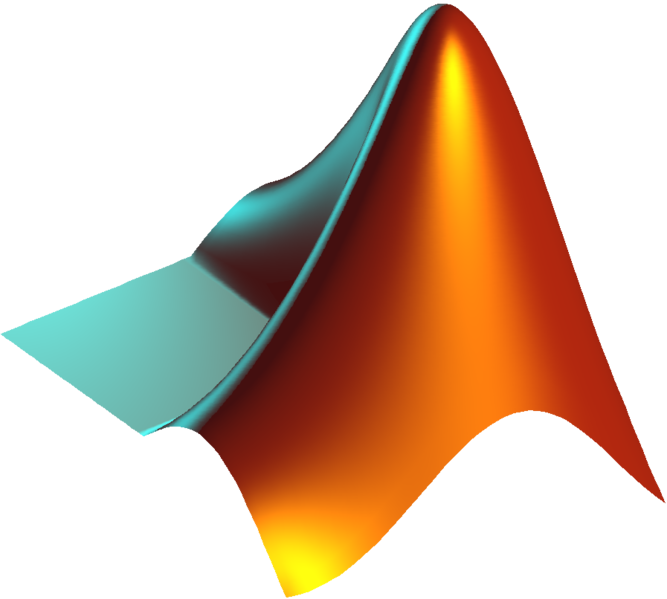
\includegraphics[width=0.05\textwidth]{logoMatlab} & 
    \raisebox{.5\height}{
\includegraphics[width=0.05\textwidth]{logoLatex}} & 
    
\includegraphics[width=0.05\textwidth]{logoMsOffice} \\
    \end{tabular}
\end{table}\\


\end{rSection}

%-------------------------------------------------
%	KEY ACCOMPLISHMENTS SECTION
%-------------------------------------------------

%-------------------------------------------------
%	EXTRA-CURRICULAR SECTION
%-------------------------------------------------

%-------------------------------------------------
%	PERSONAL INFORMATION SECTION
%-------------------------------------------------

\begin{rSection}{PERSONAL INFORMATION}

\begin{tabular}{ @{} >{\bfseries}l @{\hspace{6ex}} l }
Date of Birth & 22 November 1994\\
Marital status & Unmarried.\\
Languages known & English and Spanish.\\
Special interests & Music, mountain biking, hiking, \\
\end{tabular}

\end{rSection}

\end{document}
